\autobookmark
\begin{frame}{Current tools can not handle the dimensions of upcoming lasers}
  \begin{columns}[c]

    \begin{column}{.3\textwidth}
      \begin{center}
        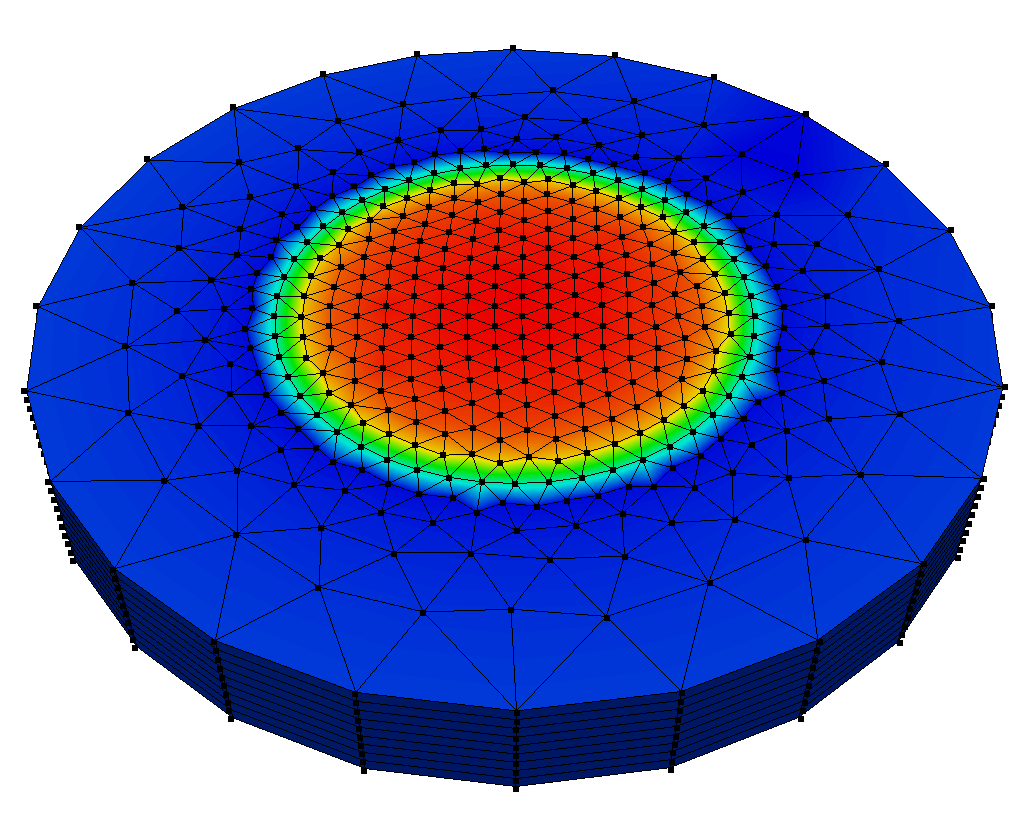
\includegraphics[width=0.1\paperwidth]{graphics/gain_medium_ASE.png}\\
        $\Downarrow$\\
        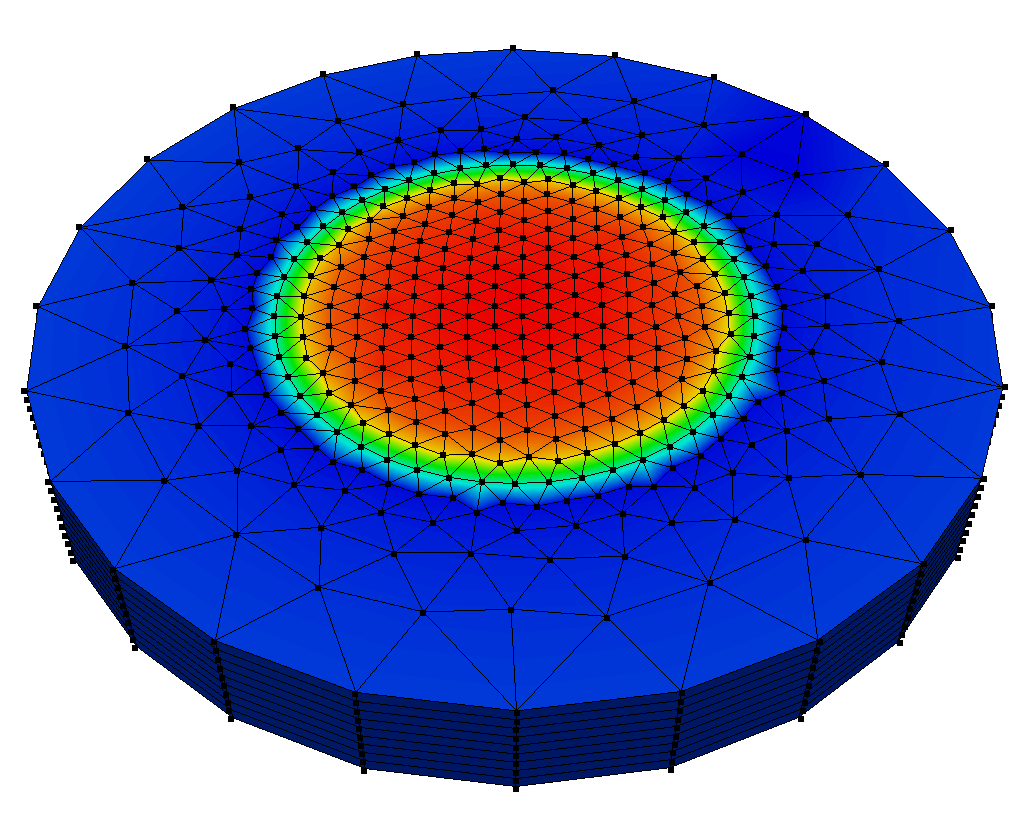
\includegraphics[width=0.3\paperwidth]{graphics/gain_medium_ASE.png}
      \end{center}
    \end{column}

    \begin{column}{.7\textwidth}
      \begin{itemize}
          \myuncover{1}{3}{
          \item With current software, it takes a long time to simulate ASE
            with a high spatial resolution\\[1ex]
          }
          \myuncover{2}{3}{
          \item Gain media are getting bigger and bigger, which makes the
            problem even worse\\[1ex]
          }
          \myuncover{3}{3}{
          \item We developed a fast tool to simulate ASE\\[1ex]

          \item Allows to simulate the full problem, instead of estimating ASE
            with a simplified model
          }
      \end{itemize}
    \end{column}

  \end{columns}
\end{frame}

%\begin{frame}{Predefined colours}
%  The template defines a set of colours according to the CD guidelines:\par
%  \begin{itemize}
%      \begin{minipage}[t]{0.5\linewidth}
%      \item \textcolor{hzdr-blue}{Helmholtz Blue}    
%      \item \textcolor{hzdr-orange}{Rossendorf Orange}  
%      \item \textcolor{hzdr-darkblue}{Helmholtz Dark Blue}
%      \item \textcolor{hzdr-gray1}{Gray1}   
%      \item \textcolor{hzdr-gray2}{Gray2}   
%      \item \textcolor{hzdr-gray3}{Gray3}   
%      \item \textcolor{hzdr-struct}{Structure of Matter}  
%      \end{minipage}%
%      \begin{minipage}[t]{0.5\linewidth}
%      \item \textcolor{hzdr-health}{Health}  
%      \item \textcolor{hzdr-energy}{Energy}  
%      \item \textcolor{hzdr-earth}{Earth and Environment}   
%      \item \textcolor{hzdr-keytec}{Key Technologies}  
%      \item \textcolor{hzdr-aero}{Aeronautics, Space and Transport}
%      \end{minipage}
%  \end{itemize}
%\end{frame}

